\Chapter{A gépi játékos megvalósítása}

Itt történik az elkészült szoftver megvalósításának bemutatása, az előző fejezetben leírt terv szempontjai alapján.

\Section{Architektúra}

Mielőtt elkezdenénk részletezni az egyes elemek konkrét realizációját, érdemes egy pillantást venni, hogy hogyan is áll össze az egész rendszer, amelyet \aref{fig:rect}. ábra szemléltet. 

\begin{figure}[h]
    \centering
    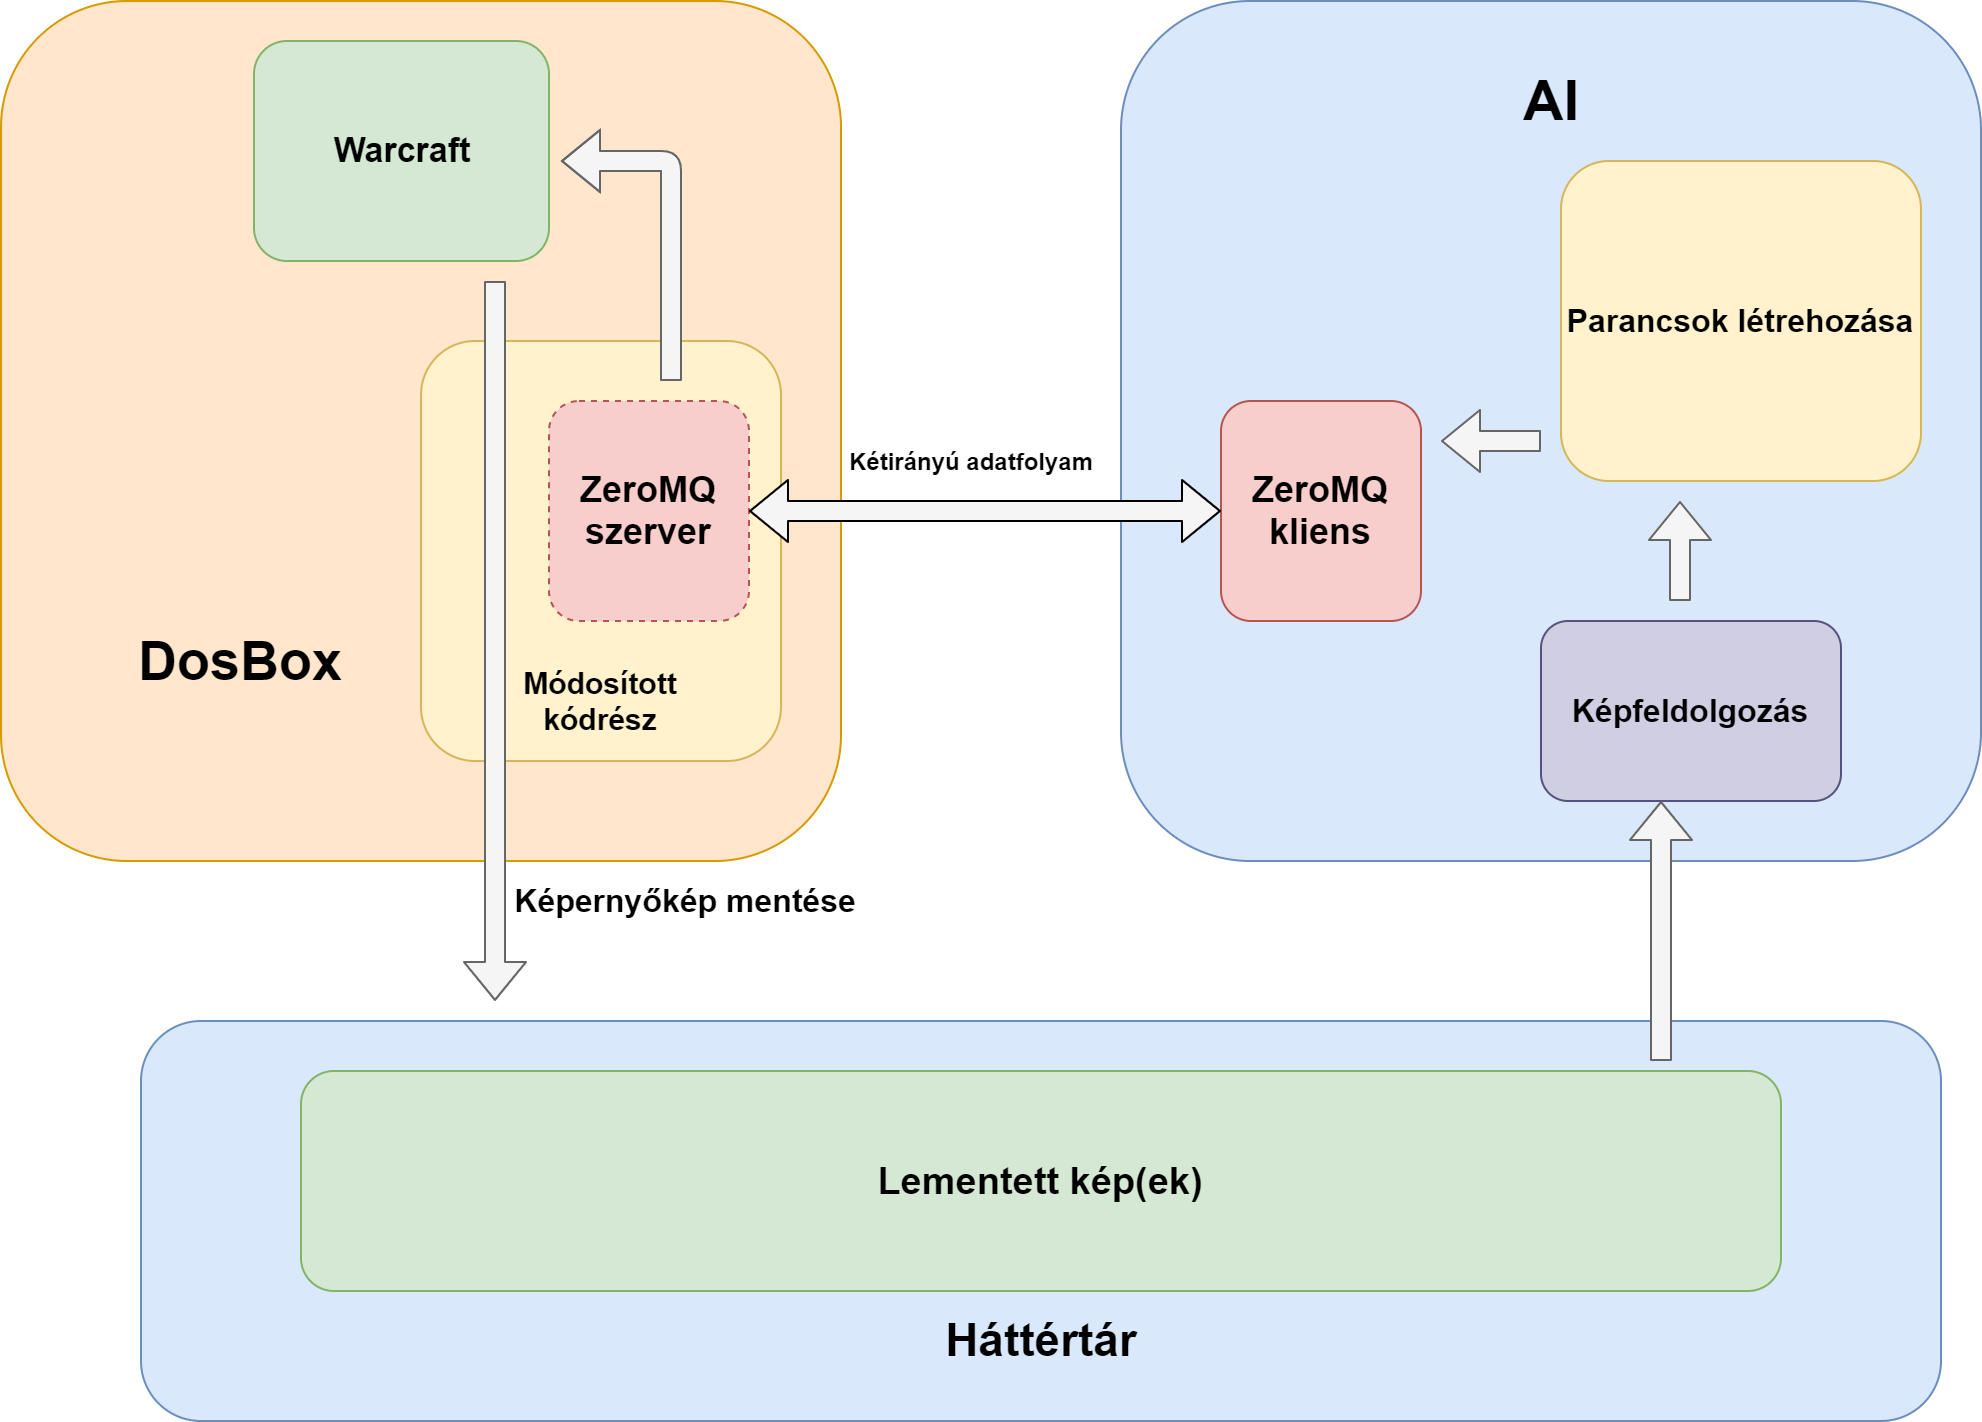
\includegraphics[scale=0.22]{images/architecture.png}
    \caption{Az elkészült alkalmazás architektúrája}
    \label{fig:rect}
\end{figure}

Az üzenetek amiket a ZeroMQ kliens küld, azok lényegében azt tartalmazzák, hogy hova kell kattintani. 
Vannak "atomi" parancsok, például a sima \textit{click} parancs, ugyanakkor léteznek bonyolultabbak, mint a \textit{geather}, ami több atomi utasításból áll. Természetesen minden parancshoz meg kell adni a kattintás pontos koordinátáját, összetett parancsnál többet is. Ez azért is jó mert elméletileg minden bonyolultabb utasítás megoldható atomi utasításokkal, ugyanakkor a teljesítmény növelése érdekében lettek létrehozva az összetett utasítások, mert az egyetlen egy adatküldés során létrejön, míg külön-külön küldve ez sokkal több.

Nagyon jól látható a modularitás ami a rendszerben van, ugyanis bármilyen más kliens is képes lehet üzenetet küldeni a DosBox-ban található szerverre, amennyiben tisztában van a lehetséges parancsokkal. Ez megkönnyíti a további alkalmazások készítését, és a felhasználási területet is. Az is látszik, hogy az egész Warcraft-ot lényegében körbe zárja a DosBox, így csak azon keresztül lehet vele interakcióba lépni. 

\Section{DosBox}

\SubSection{Buildelés}

Első lépésként a forráskódot kell beszerezni, ez a fejlesztés ideje alatt elérhető legfrissebb verzióban történt meg. (A további frissítése új verziókra csak abban az esetben indokolt ha kritikus hibát találok a fejlesztés során, egyébként csak komplikációk adódnának miatta.)
% ref: https://sourceforge.net/p/dosbox/code-0/4392/tree/dosbox/

A következő lépés a beszerzett forráskód buildelése. Mivel jelenleg a Windows-t használom gyakrabban, így a DosBox buildelése, és a mesterséges intelligencia is Windows alatt készült. Nem kizárt, hogy Linux alatt is elinduljon mind a DosBox, mind az MI, de a szakdolgazat nem foglalkozik erre az operációs rendszerre történő optimalizálással.
% ref: https://www.dosbox.com/wiki/Building_DOSBox_with_Visual_Studio

Ha megpróbálnánk így lefordítani, azonnal hibába ütköznénk, ugyanis szükségesek hozzá különböző könyvtárak.

\begin{itemize}

    \item SDL (Simple DirectMedia Layer)
    
    Az egyetlen kötelező könyvtár és talán legfontosabb. Az SDL egy több platformos fejlesztői könyvtár, amelyet arra találtak ki, hogy alacsony szintő hozzáférést biztosítson többek között az egérhez, billentyűzethez, különböző játékvezérlőkhöz, magához a hanghoz OpenGL és Direct3D segítségével. Rengeteg híres videojáték használja ezt a technológiát. Sajnos a DosBox elég válogatós, így a leírás alapján nem a legfirsebb verziót kéri, hanem egy jóval régebbi kiadást.
    \item zlib / libpng (opcionális)
    
    Egy opcionális könyvtár képek és videók mentésére. A tervben vázoltak alapján arra következtetünk, hogy ez még a hasznunkra vállhat, így mind a két könyvtárat is le kell töltenünk, mivel a \textit{libpng} követelménye a \textit{zlib}. 
    \item SDL\_net (opcionális)
    
    Lehetővé teszi a hálózat használatát. A többjátékos mód eléréséhez elengedhetetlen, ugyanakkor nincs tervben ennek a használata. Amennyiben ez módosul, ezt is hozzáadjuk a könyvtárakhoz.
    \item SDL\_sound (opcionális)
    
    Lejátszhatóak lesznek a tömörített hanggal rendelkező CD-k.
    \item PDCurses (opcionális)
    
    Elérhetővé teszi a DOS Debuggert.

\end{itemize}

Miután eldöntöttük mely könyvtárak szükségesek nekünk a fordításhoz, a fordítási útmutató alapján beállítjuk a linkereket megfelelően, és a szükséges DLL fájlokat is. 

Utolsó dolgunk átírni a \textit{config.h} nevű fájlban az alábbi konfigurációkat: 

\begin{cpp}

    ...
    #define C_DEBUG 0 // PDCurses

    #define C_SSHOT 1 // libpng

    #define C_SRECORD 1 // zlib

    #define C_MODEM 0 // SDL_net 

    #define C_IPX 0 // SDL_net 
    ...
\end{cpp}

\SubSection{DosBox átalakítása - bemenetek}

Ahhoz hogy a tervben leírtakat meg tudjuk valósítani, meg kell találnuk a számunkra fontos kódrészeket. Ezek sorrendtől függetlenül a következők:
\begin{itemize}
    \item egér,
    \item billentyűzet,
    \item képernyőkép.
\end{itemize}

A fájlok közül rákereshetünk hogy tartalmazza-e valamelyik a \textit{keyboard} vagy \textit{mouse} kulcsszavatak. Ezekre rákeresve találunk 2 fájlt ami számunkra érdekes lehet. Az egyik a \textit{keyboard.h} a másik a \textit{mouse.h}.

Így néz ki például a \textit{keyboard.h} header fájl:

\begin{cpp}
    #ifndef DOSBOX_KEYBOARD_H
    #define DOSBOX_KEYBOARD_H
    
    enum KBD_KEYS {
        KBD_NONE,
        KBD_1,	KBD_2,	KBD_3,	KBD_4,	KBD_5,	KBD_6,	KBD_7,	
        KBD_8,	KBD_9,	KBD_0,		
        KBD_q,	KBD_w,	KBD_e,	KBD_r,	KBD_t,	KBD_y,	KBD_u,	
        KBD_i,	KBD_o,	KBD_p,	
        KBD_a,	KBD_s,	KBD_d,	KBD_f,	KBD_g,	KBD_h,	KBD_j,	
        KBD_k,	KBD_l,	KBD_z,
        KBD_x,	KBD_c,	KBD_v,	KBD_b,	KBD_n,	KBD_m,	
        KBD_f1,	KBD_f2,	KBD_f3,	KBD_f4,	KBD_f5,	KBD_f6,	KBD_f7,	
        KBD_f8,	KBD_f9,	KBD_f10,KBD_f11,KBD_f12,

        ...
        
    };
    
    void KEYBOARD_ClrBuffer(void);
    void KEYBOARD_AddKey(KBD_KEYS keytype,bool pressed);
    
    #endif
\end{cpp}

Látható, hogy a különböző billentyűk egy felsorolásban (\textit{enum}) vannak tárolva, általános alakját tekintve \textit{KBD\_KEY}.
Továbbá a fájl végén található egy függvény fejléce:

\begin{cpp}
    void KEYBOARD_AddKey(KBD_KEYS keytype,bool pressed);
\end{cpp}

Itt látható, hogy ez a függvény paraméterbe kér egy billentyűt, a fentebb látott enum-ból, majd egy igaz/hamis értéket, hogy le van-e nyomva avagy sem. Ebből tisztán látszik, hogy amennyiben meghívjuk ezt a függvényt egy gombra igaz paraméterre, majd közvetenül utána hamissal, gomblenyomást tudunk szimulálni kódon belül. 

Ezzel a billentyűzethez hozzá tudunk férni igen egyszerűen, következhet is az egér, amelyet a \textit{mouse.h} header fájlban találunk.

\begin{cpp}

    #ifndef DOSBOX_MOUSE_H
    #define DOSBOX_MOUSE_H
    
    
    void Mouse_ShowCursor(void);
    void Mouse_HideCursor(void);
    
    bool Mouse_SetPS2State(bool use);
    
    void Mouse_ChangePS2Callback(Bit16u pseg, Bit16u pofs);
    
    void Mouse_CursorMoved(float xrel,float yrel,
                           float x,float y,bool emulate);

    void Mouse_CursorSet(float x,float y);
    void Mouse_ButtonPressed(Bit8u button);
    void Mouse_ButtonReleased(Bit8u button);
    
    void Mouse_AutoLock(bool enable);
    void Mouse_BeforeNewVideoMode(bool setmode);
    void Mouse_AfterNewVideoMode(bool setmode);
    
    #endif

\end{cpp}

Itt már nehezebb dolgunk van mint a billentyűzetnél. Vannak ugyan egyszerűbb fügvények is, mint például a \verb|Mouse_ShowCursor(void)| és a \verb|Mouse_ShowCursor(void)| amelyekkel el lehet tűntetni, majd ismét meglejeníteni a kurzort,
És a\\ \verb|Mouse_CursorSet(float x,float y)| működése is evidens, a képernyő 2 koordinátáját kell megadni és a kurzort oda rakja.

Ennél bonyolultabb függvény a \verb|Mouse_ButtonPressed(Bit8u button)| és a hozzá tartozó \verb|Mouse_ButtonReleased(Bit8u button)|. A használatát tekintve első ránézésre hasonlónak tűnik mint a billentyűzetnél lévő függvény. Ugyanakkor mivel a \textit{Bit8u} nem egy alapértelmezett típus, érdemes betekinteni a függvény definíciójába, hogy pontosan megértsük mit is vár el paraméternek.

Vegyük például a gomb lenyomásához tartozó függvényt:
\begin{cpp}

    void Mouse_ButtonPressed(Bit8u button) {
            switch (button) {
        #if (MOUSE_BUTTONS >= 1)
            case 0:
                if (mouse.buttons&1) return;
                mouse.buttons|=1;
                Mouse_AddEvent(MOUSE_LEFT_PRESSED);
                break;
        #endif
        #if (MOUSE_BUTTONS >= 2)
            case 1:
                if (mouse.buttons&2) return;
                mouse.buttons|=2;
                Mouse_AddEvent(MOUSE_RIGHT_PRESSED);
                break;
        #endif
        #if (MOUSE_BUTTONS >= 3)
            case 2:
                if (mouse.buttons&4) return;
                mouse.buttons|=4;
                Mouse_AddEvent(MOUSE_MIDDLE_PRESSED);
                break;
        #endif
            default:
                return;
            }
        mouse.times_pressed[button]++;
        mouse.last_pressed_x[button]=POS_X;
        mouse.last_pressed_y[button]=POS_Y;
    }

\end{cpp}

Látható, hogy annak fügvényében, hogy mennyi gomb található az egéren (alapértelmezetten 3), az alapján engedélyez különböző eseteket a program. Alapértelmezett esetben az alábbiakra tudunk következtetni:
\begin{itemize}
    \item ha a \textit{button} paraméter értéke 0, az a bal egérgombnak felel meg,
    \item amennyiben az értéke 1, akkor az a jobb egérgomb,
    \item amennyiben az érték 2, akkor az a görgő lenyomása.
\end{itemize}
Ezt kombinálva a gomb eleresztésével láthatóvá válik, hogy ugyan úgy képesek vagyunk kattintani 2 függvény meghívásával, mint ahogyan ezt a billentyűzetnél tettük.

\SubSection{Dosbox átalakítása - képernyőkép}

További fontos, ugyanakkor nehezebb probléma a képernyő képének lementése. Első lépésként meg kell találni a az ehhez szükséges függvényt vagy függvényeket. 
A \textit{screenshot} szóra rákeresve a fájlok között a \textit{hardware.cpp}-ben találunk egy\\ \verb|CAPTURE_ScreenShotEvent| nevű függvényt, ugyanakkor ez nem paraméterezhető megfeleően, csak egy igaz/hamis értéket lehet megadni benne. 
Tovább böngészve ugyan ebben a fájlban megtalálhatjuk a \verb|CAPTURE_AddImage| függvényt, mely számos paraméterrel rendelkezik, a függvény definíciójában pedig megtalálható a menteni kívánt fájl kiterjesztése is.

Ezek után olyan részt kell találni a kódban, ahol periodikusan lehet futtatni az általunk megírt logika alapján a kép lementését anélkül, hogy lassítanánk a szoftver futását. Erre hosszadalmas keresés után a \textit{render.cpp} \verb|RENDER_EndUpdate| függvénye tűnik alkalmasnak, mivel ez a függvény minden frame végén lefut. 
A függvény végét az alábbi kóddal bővítettem ki:
\begin{cpp}
    if(1)
    {
        ...

        if (fpsCounter >= render.src.fps)
        {
            CAPTURE_AddImage(render.src.width==0?640:render.src.width, 
                             render.src.height==0?400:render.src.height, 
                             render.src.bpp, pitch,
                             flags, fps, (Bit8u*)&scalerSourceCache, 
                             (Bit8u*)&render.pal.rgb);
            CaptureState = 0;
            fpsCounter = 0;
        }
    
        else
        {
            fpsCounter++;
        } 
    }
\end{cpp}
Ennek a lényege, hogy létrehozunk egy belső FPS számlálót, és minden frameben összehasonlítjuk az elvárt FPS-el, amennyiben ezt elértük vagy túlhaladtunk rajta, lementjük a képernyő jelenlegi tartalmát.
Ezzel technikailag másodpercenként lehet képernyőképet csinálni. Ezzel a módszerrel ez a lehető legrövidebb intervallum.

\SubSection{Dosbox átalakítása - ZeroMQ}

Miután elkészült a képernyőkép bizonyos időközönkénti mentése, egy újabb nehezebb feladat következik. Implementálnunk kell a tervben leírt processzek közötti kommunikációt. 
Erre a már szintén említett \textit{ZeroMQ} lesz a segítségünkre, amit először tesztelnünk kell C++ban és Pythonban egyaránt.

Mielőtt konkrétan beágyaznánk bármiféle kódot a DosBoxba, nézzük meg hogyan is működik egy egszerű \textit{request-reply} alapján.
\begin{python}
import zmq
import time

context = zmq.Context()

#  create socket
print("Connecting to server...")
socket = context.socket(zmq.REQ)
socket.connect("tcp://localhost:5555")

#  Do 10 request and wait for reply
for request in range(10):
    print("Sending request %s ..." % request)
    msg = input("message: ")
    socket.send(bytes(msg))

    
    #  Get the reply.
    message = socket.recv()
    print("Received reply %s [ %s ]" % (request, message))
\end{python}
Itt az látható, hogy létrehozunk egy kontextust, majd ebből egy socketet melynek a \textit{request} típust adjuk. 
Utána megadjuk a kapcsolat típusát, címét és a portot. Ebben a mintában 10 üzenetet tudunk küldeni, amit byte sorozatként küldi el, és minden üzenet után megvárjuk a választ. Ez lényegében a kliensünk, a következő, már C++ban írt kód pedig a szerver lesz, ami fogadja az üzeneteket és választ ad rájuk.
\begin{cpp}
#include <zmq.hpp>
#include <string>
#include <iostream>
#include <windows.h>
int main()
{
    zmq::context_t context(1);
    zmq::socket_t socket(context, ZMQ_REP);
    socket.bind("tcp://*:5555");

    while (true) {
        zmq::message_t request;

        //  Wait for request
        socket.recv(&request);
        std::cout << "Received " << request.to_string() << std::endl;

        //  Do some 'work'
        Sleep(1);

        //  Send reply 
        zmq::message_t reply(5);
        memcpy(reply.data(), "Hello", 5);
        socket.send(reply);
    }
    return 0;
}
\end{cpp}
Felépítést tekintve nagyon hasonló a az előző kódhoz, de mivel szerverként funkcionál, így üzenetre vár, majd aztán küld egy válasz üzenetet. 

Értelemszerűen ezt a kódrészt kell a DosBoxba integrálni míg az előzőt a mesterséges intelligenciába kell beágyazni. Először megkeressük azt a kódrészt ahová ezt, vagy ennek egy módosított változatát be tudjuk integrálni. Jó gondolat a jól megszokott \textit{render.cpp}-be történő bővítés, ugyanis folyamatosan figyelni kell az üzenetet és reagálni rá. Viszont ezt kipróbálva abba a problémába ütközünk, hogy a program addig "lefagy" amíg nem kap üzenetet. Ez ividens, ugyanis a \verb|socket.recv(&request)| sor lényege, hogy addig vár, amíg nem kap üzenetet. Ezt egy végtelen ciklusba rakva láthatóvá válik mi is a gond.

Ennek kiküszöbölése érdekében egy külön függvényben kell definiálni a szerver kódját, majd egy új szálat indítani, és ennek párhuzamosan kell futnia a program többi részével. Így nem fagy le a programunk, és a fentebb leírt periféria manipuláló függvényeket is meg tudjuk hívni.
\begin{cpp}
void ZeroMQLoop()
{
    zmq::context_t context(1);
    zmq::socket_t socket(context, ZMQ_REP);
    socket.bind("tcp://*:5555");

    while (true) {
        zmq::message_t request;

        //  Wait for next request from client
        socket.recv(&request);
        LOG_MSG(request.to_string().c_str());

        std::vector<std::string> result;
        std::istringstream iss(request.to_string());
        for (std::string s; iss >> s; )
            result.push_back(s);

        if (result[0] == "Click")
        {
            // Click code
        }
        else if (result[0] == "Move")
        {
            // Move code
        }

        else if (result[0] == "Gather")
        {
            // Gather code
        }
        else if (result[0] == "Attack")
        {
            // Attack code
        }
        else if (result[0] == "Start")
        {
            // Start code
        }

        //  Send reply back to client
        zmq::message_t reply(5);
        memcpy(reply.data(), "Done", 4);
		
        socket.send(reply);
	}
}
\end{cpp}

\Section{AI megvalósítása}

A DosBox módosítása után a konkrét program megírása következik. A legjobb megoldás ehhez az, ha egy külön osztályt készítünk az AI-nak, és annak definiáljuk az adattagokat és metódusokat. Ehhez fel kell írni hogy mégis milyen adatokra van szükség.
\begin{itemize}
    \item Tudni kell hogy az egyes nyersanyagokból éppen mennyi áll rendelkezésre
    \item A térkép jelenlegi állását/állásait is le kell menteni
    \item Elvégzendő parancsok listája
    \item Kapcsolat a DosBox-al
\end{itemize}
Természetesen a lista nem teljes, fejlesztés során bővülhet, de a legfontosabb dolgokat tartalmazza

\SubSection{Működés részletes leírása}

Ezt követően létre kell hozni a kapcsolatot az "agy" és a "test között". Ugyanis technikailag a "gondolkodást" a Python-ban írt AI fogja véghez vinni, elküldeni a teendőket a DosBoxna, majd az végrehajtja. Az adatok küldéséhez az előző pontban leírt
ZeroMQ-s megoldást fogjuk használni. Az AI osztályunk példányosítása után, a \textit{Start()} metódussal indítható, és a \textit{Stop()} metódussal állítható meg. 

A végtelen ciklust itt is érdemes megtartani, ugyanis nem tudhatjuk meddig szeretné a felhasználó használni a programot, és szinte másodpercenként üzenetet kell továbbítania, így ezért sem előnyös leállítani. Az egyszerű
leállítás érdekében ugyanakkor a ciklust egy try blokkban definiáltam, ami kivételt dob amennyiben a felhasználó billentyűzet megszakítást küld (példálul ctrl+c a terminálban) a program elkezdi a leállás folyamatát, megszakítja a kapcsolatot a DosBoxal és leáll.

Ennek függvényében nézzük meg milyen lépései \aref{fig:lepesek}. ábrán láthatóak.

\begin{figure}[h]
    \centering
    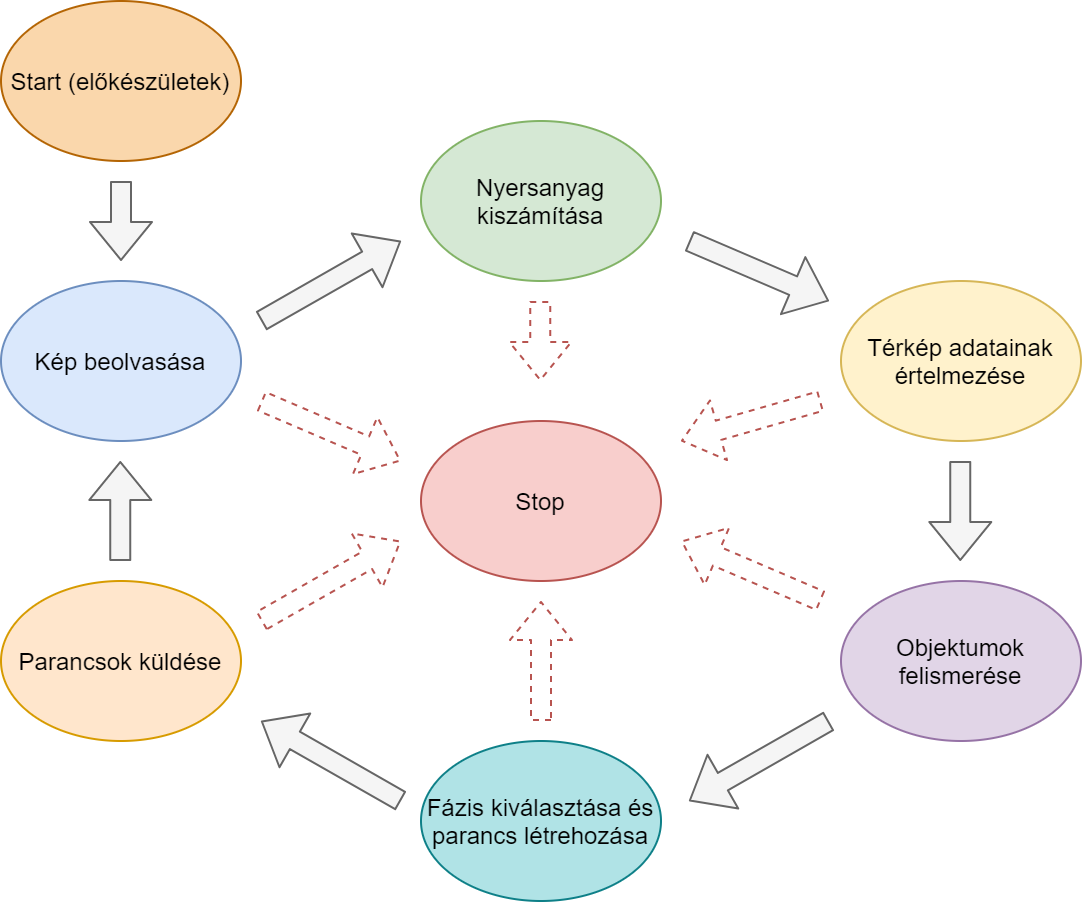
\includegraphics[scale=0.4]{images/image0.png}
    \caption{Végrehajtandó lépések}
    \label{fig:lepesek}
\end{figure}

Észrevehető a ciklikusság, továbbá az is, hogy a program terminálódása életciklusának bármelyik szakaszában bekövetkezhet, amikor is megszakítást kap a felhasználótól.

Az összképet látva, első dolgunk, még mielőtt bármiféle logikát be tudnánk programozni, a tervben szereplő adatfeldolgozás létrehozása, azaz lementett képből kell olyan használható adatokat kinyerni, amelyek segítségével konkrét parancsot lehet előállítani. 
A beolvasáshoz a config fájlban használt elérési útvonalat tudjuk használni, így könnyen változtathatóak.

Alapértelmezett konfigurációs fájl:
\begin{python}
class Config:
    tesseract = r".\TesseractOCR\tesseract.exe"
    capture = r".\capture\war_000.png"
\end{python}

Kép beolvasása:
\begin{python}
    ...

    while self.loop:

        ... 
        
        image = cv2.imread(Config.capture)

        ...
\end{python}

Egy beolvasott kép \aref{fig:abra}. ábrán látható formában néz ki.

\begin{figure}[h]
\centering
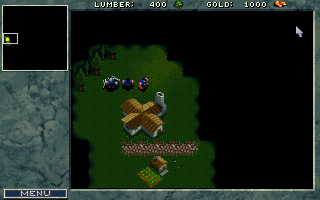
\includegraphics[scale=1]{images/war_000.png}
\caption{Egy DosBox által lementett kép.}
\label{fig:abra}
\end{figure}

Beolvasás után jöhet az adatok kinyerési. Itt van egy kis szabadságunk a tekintetben, hogy mivel kezdünk. Úgy gondoltam a nyersanyagok számának meghatározását veszem előre. A függvény bemenetként a nyersanyag nevét kéri, és ndarray-t, 
ami lényegében a beolvasott kép azon szelete ahol az adott nyersanyag található.
Maga a függvény így néz ki:
\begin{python}
def ReadText(self, name: str,cropImage: np.ndarray):

    if cropImage is None:
        return

    scale_percent = 600 
    width = int(cropImage.shape[1] * scale_percent / 100)
    height = int(cropImage.shape[0] * scale_percent / 100)
    dimension = (width, height)


    res = cv2.resize(cropImage, dimension, 
                    interpolation = cv2.INTER_AREA)
    gray = cv2.cvtColor(res, cv2.COLOR_BGR2GRAY)

    thresh = cv2.threshold(gray, 200, 255, 
                        cv2.THRESH_BINARY + cv2.THRESH_OTSU)[1]

    skeleton = cv2.threshold(thresh,0,1,cv2.THRESH_BINARY)[1]
    skeleton = (255*skeletonize(skeleton)).astype(np.uint8)
    kernel = cv2.getStructuringElement(cv2.MORPH_ELLIPSE, (4,6)) 
    skeleton_dilated = ~cv2.morphologyEx(skeleton, 
                            cv2.MORPH_DILATE, kernel)

    data = pytesseract.image_to_string(skeleton_dilated, 
    lang='eng', config='--psm 10 -c tessedit_char_whitelist=0123456789s')
    print(f"{name}: "+data.replace("\$","8").replace("o","0")
                    .replace("s","5").replace("i","1"))

    cv2.imwrite(f"{name}.png",skeleton_dilated)
\end{python}

Szinte sorról sorra magyarázva ez azt csinálja, hogy először megnézzük létezik-e ez a kép részlet, amennyiben nem, a függvény azonnal visszatér. Ezt azért tehetjük meg, mert másodpercenként minimum egyszer frissülnek az adatok, így nem probléma ha néha-néha kimarad egy ilyen frissítési ciklus, és így a program is fut tovább ahelyett hogy hibát dobna.
Először megadjuk a nagyítás mértékét, ez több próbálkozás után lett 600\%-os, mivel ez bizonyult a legjobbnak. Kiszámoljuk az így kapott hosszt és szélességet, majd a \textit{dimension} változóba eltároljuk későbbi használatra. 
A \textit{res} változóban lesz maga kivágott kép nagyított változata, amihez a \textit{cv2.INTER\_AREA} interpolációját használjuk, ami a képek nagyítását szolgálja.

Annak érdekében hogy a \textit{tesseract} képes legyen felismerni a számokat, a színes képet érdemes szürkeárnyalatos képpé alakítani alakítani, ezt a \textit{gray} változóba tároljuk a \textit{cv2.cvtColor} függvény segítségével, aminek a használata elég egyszerű
megadjuk a módosítani kívánt képet, és a módosítást. Ez esetben ez a \textit{cv2.COLOR\_BGR2GRAY} lesz, amivel egyszerűen elérhető a kívánt eredmény.
Habár a szürke árnyalatos kép hatalmas előrelépés, egy küszöbérték függvény is érdemes alkalmazni amivel ki tudjuk emelni a számunkra fontos adatokat a képen, ami ez esetben maga a szám (\ref{fig:orig}. ábra).

% ref: https://www.geeksforgeeks.org/python-thresholding-techniques-using-opencv-set-1-simple-thresholding/

\begin{equation*}
    output(x, y) = \left\{ 
    \begin{matrix}
        max, & \text{ha } input(x, y) > thres, \\
        0, & \text{egyébként}.
    \end{matrix} \right.
\end{equation*}

Ennek az inverze

\begin{equation*}
    outputinv(x, y) = \left\{ 
    \begin{matrix}
        0, & \text{ha } input(x ,y) > thres, \\
        max, & \text{egyébként}.
    \end{matrix} \right.
\end{equation*}

\begin{figure}[h]
    \centering
    
\includegraphics[scale=1]{images/grey.png}
    
\includegraphics[scale=1]{images/thres.png}
    \caption{Szürkeárnyalatos (bal) és küszöbértékes (jobb) kép.}
    \label{fig:orig}
\end{figure}

A következő lépés az úgynevezett \textit{skeletonization} {\cite{skeletonization}}, aminek lényege a kép "vázának" megjelenítése és élesítese a háttér és egyéb nem fontos információ nélkül, továbbá mivel az eredeti kép "pixeles", valahogyan le kell kerekíteni hogy a Tesseract könnyebben felismerje, a skeletonization ebben is a segítségünkre van. Utolsó lépésnek invertálni kell a képet, hogy a szám az fekete legyen, ezt a \textit{~} karakter segítségével tehetjük meg.

A fájlba mentés opcionális, mivel nem kell beolvasni, de megnyitva például \aref{fig:numbers}. ábrán látható eredményt találjuk.

\begin{figure}[h]
    \centering
    
\includegraphics[scale=1]{images/Lumber.png}
    
\includegraphics[scale=1]{images/Gold.png}
    \caption{Bal oldalon a jelenlegi fák száma látható, míg jobb oldalon az arany száma. }
    \label{fig:numbers}
\end{figure}

Ahogyan a nyersanyagok adatait, úgy a térkép adatait is le kell menteni. Ha térkép lemérése után azt tapasztaljuk hogy a mérete 64x64, ahol egy pixel egy tile-t jelent, azaz ezen csak egyetlen egy egység állhat. Az épületek ennél bonyolultabbak, ugyanis a méretük lehet 2x2 vagy 3x3 is, 
de ez sem okoz akkora problémát, nyugodtan feloszthatjuk a térképet 64x64 mezőre. Nem előnyös ugyanakkor minden információt egy 64x64 méretű listában/tömbben tárolni, így az információ típusától függően 3 csoportra osztottam.
\begin{itemize}
    \item Nyersanyag térkép: csak a nyersanyagokat és a munkásokat tárolja.
    \item Felfedező térkép: azt az értéket tárolja hogy fel van-e fedezve az adott mező vagy sem, továbbá a saját és az ellenséges katonákat is (például, mint ahogy \aref{fig:map}. ábrán látható).
    \item Épület térkép: A felépült épületeket és utakat tárolja.
\end{itemize}


\begin{figure}[h]
    \centering
    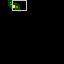
\includegraphics[scale=2]{images/map.png}
    \caption{A térkép kivágva, ahogyan a program dolgozik vele}
    \label{fig:map}
\end{figure}

\begin{python}
def UpdateMap(self,cropMap):
    self.offset = self.GetOffset(cropMap)
    for i in range(64):
        for j in range(64):
            if(list(cropMap[i][j]) == [0,0,0]):
                self.map[1][i][j] = -1
            elif(list(cropMap[i][j]) == [0,0,255]):
                self.map[2][i][j] = 100
            elif(i+1 != 64 and j+1 != 64 
            and list(cropMap[i][j]) == [199,199,199] 
            and list(cropMap[i+1][j]) == [199,199,199] 
            and list(cropMap[i+1][j+1]) == [199,199,199] 
            and list(cropMap[i][j+1]) == [199,199,199]):
                self.map[0][i][j] = 3    
\end{python}

A térkép frissítése a fentebb látható kód alapján történik. Itt lényegében pixelenként át kell nézni a képet, majd az adott szín alapján következtetésrekre jutni és az adott lista adott elemébe betölteni a megfelelő értéket.

Miután a térképről kinyertük a szükséges adatokat, ideje a játéktérre fókuszálni, itt látható ugyanis a térkép egy 15x11 mező méretű szelete, ahol tudjuk az egységeket irányítani, nyersanyagokat szerezni, és építeni.
Egy mező mérete 16x16 pixel, ugyanakkor ugyan ez a mező a térképen 1x1 pixelt jelentett, így jön az ki, hogy a játéktér 15x11 mezőt foglal magában, amit az alábbi kép is alátámaszt.
\begin{figure}[h]
    \centering
    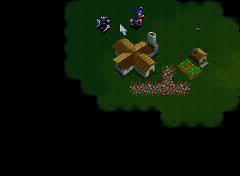
\includegraphics[scale=0.8]{images/playArea.png}
    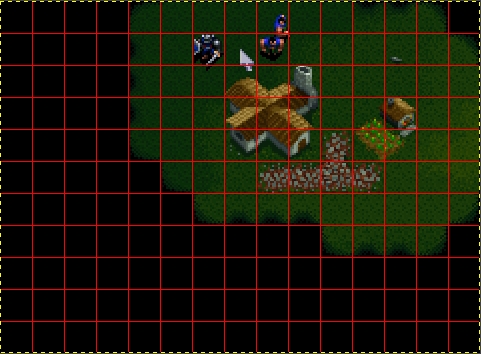
\includegraphics[scale=0.53]{images/playAreaRed.png}
    \caption{Játéktér rácsok nélkül (bal) és rácsokkal (jobb)}
    \label{fig:playArea}
\end{figure}

Itt szépen kivehető, hogy egy egység 1 mezőt foglal el, és pontosan illeszkedik ré (kivéve mozgáskor, de ez elhanyagolható), az épületek és utak körvonala is tisztán látszik hogy szabályos (\ref{fig:playArea}. ábra).
Ebből arra a következtetésre lehet jutni, hogy a játéktéren belül is érdemes mezőnként átnézni a képet és az adott 16x16-os blokkon belül érzékelni hogy milyen típusú objektumot találtunk.

Ehhez egy \textit{Unit} segédosztály hozunk létre, ami megadja az általános formáját az eltárolni kívánt objektumnak.

\begin{python}

class Unit:
    def __init__(self,unit_id,location,color,threshold,mapmode):
        self.location = location
        self.color = color
        self.threshold = threshold
        self.mapmode = mapmode
        self.unit_id = unit_id
\end{python}

Mint látható egy nagyon egyszerű, csak konstruktort tartalmazó osztályról van szó, aminek pusztán annyi lényege van, hogy a könnyebb kezelhetőség érdekében "csomagba" rakja egy adott objektumra vonatkozó összes hasznos adatot.

Az adattakok jelentései a következők.
\begin{itemize}
    \item \textit{unit id:} Megadja az egyedi azonosítót.
    \item \textit{location:} Az a hely, ahol az adott objektum spritejai vannak.
    \item \textit{color:} A keret színét adja meg.
    \item \textit{threshold:} Megadja a hibahatár mértékét. 
    \item \textit{mapmode:} Megadja melyik térképre akarjuk menteni.
\end{itemize}
Így ezt az osztályt a következő lépésben használhatjuk. Ennek a lépésnek a lényege konkrétan meghatározni hogy mit is látunk a játéktéren. Ezt egyfajta \textit{template matching}-el hajtjuk végre, melynek kódja a következő:
\begin{python}
def match_templates(self,play_area):
    img_gray = cv2.cvtColor(play_area, cv2.COLOR_BGR2GRAY)

    units = [
            Unit(1,'./imgs/footman',(255,0,0),0.85,1),
            Unit(1,'./imgs/peasant',(0,100,255),0.85,0),
            Unit(1,'./imgs/buildings',(0,255,255),0.76,2),
            Unit(2,'./imgs/tree',(19,69,139),0.8,1),
            Unit(1,'./imgs/road',(255,255,255),0.8,2)
            ]

    for unit in units:
        for filename in os.listdir(unit.location):
            
            template = cv2.imread(f"{unit.location}/{filename}",0)
            w, h = template.shape[::-1]
            for _ in ['after flip', 'before flip']:
                template = cv2.flip(template,1)
                res = cv2.matchTemplate(img_gray,template,
                cv2.TM_CCOEFF_NORMED)
                threshold = unit.threshold
                loc = np.where( res >= threshold)

                for pt in zip(*loc[::-1]):
                    if self.offset != None:
                        if(unit.mapmode == 2 and 
                            unit.location == './imgs/buildings'):
                            try:
                                self.map[unit.mapmode][self.offset[0]+
                                math.ceil(pt[1] / 16)][self.offset[1]+
                                math.ceil(pt[0] / 16)] = 
                                int(filename[:len(filename)-4])
                            except:
                                pass
                        else:
                            try:
                                self.map[unit.mapmode][self.offset[0]+
                                math.ceil(pt[1] / 16)][self.offset[1]+
                                math.ceil(pt[0] / 16)] = unit.unit_id
                            except:
                                pass
                    cv2.rectangle(play_area, pt, (pt[0] + w, pt[1] + h),
                                unit.color, 2)
                    cv2.imwrite('res.png',play_area)
\end{python}

Ismerős elemeket láthatunk a függvény elején, a képet szokás szerint szürkeárnyalatossá kell konvártálni, majd egy \textit{units} nevű listába példányosítjuk a szükséges objektumokat. Itt megjegyzendő, hogy a \textit{color} adattag fordított rgb sorrendben működik, a \textit{threshold} lényege pedig hogy hány százalékos legyen az egyezes (értelem szerűen 0 és 1 közötti értéket fogad el).

Az algoritmust minden egyes objektumra, és azoknak minden egyes változatára lefuttatjuk. Például az embereknél a \textit{footman} nevű egység lenne maga az objektum, és annak rengeteg állapota van (lefelé néz, felfelé néz, jobbra néz stb.) így azokat is ellenőrizni kell hogy rajta vannak-e a játéktéren. Továbbá a \textit{cv2.flip()} függvény
segítségével ezeknek a tükörképét is ellenőrizzük, ugyanis lehetséges hogy valamelyik mozdulatnak a tükörképe is létezik. Ez a folyamat habár hosszúnak tűnhet a sok egymásba ágyazott \textit{for} ciklus miatt, nem vesz el szignifikáns számítási időt tapasztalatom szerint, ami a kép viszonylag apró mérete miatt lehetséges. Az elemzés eredményét \aref{fig:template}. ábrán láthatjuk.

\begin{figure}[h]
    \centering
    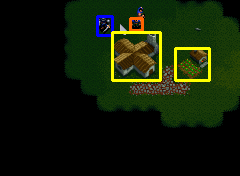
\includegraphics[scale=1]{images/res.png}
    \caption{A template matching eredménye}
    \label{fig:template}
\end{figure}
\pagebreak
Most, hogy az összes adat a rendelkezésünkre áll, ideje megnézni a fentebb beszélt fázisokat bővebben.
A lépéseket \aref{fig:phases}. ábra szemlélteti:

\begin{figure}[h]
    \centering
    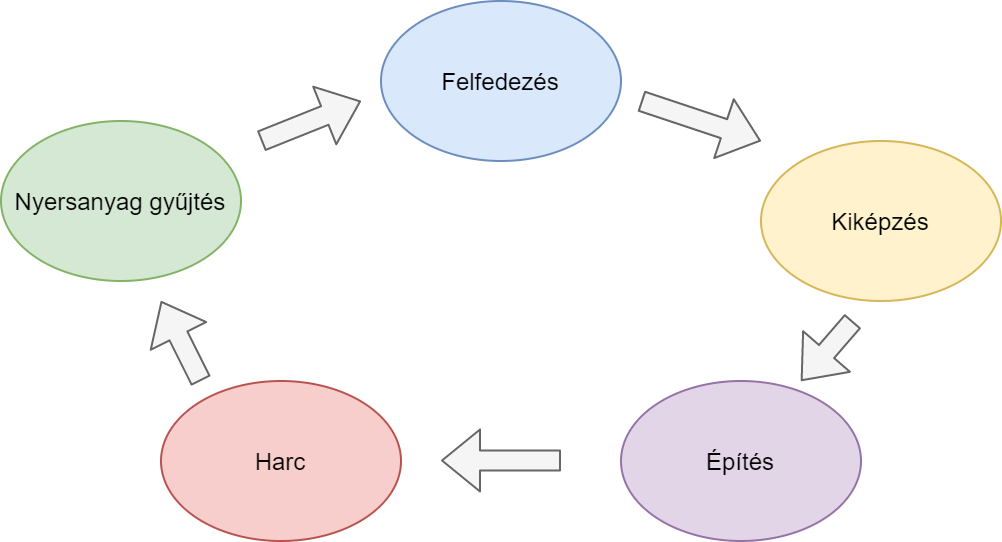
\includegraphics[scale=0.4]{images/phases.png}
    \caption{A fázisok lépései}
    \label{fig:phases}
\end{figure}

\noindent Mint látható, ez is ciklikusan történik, mégpedig úgy, hogy a ciklus elindul a nyersanyag gyűjtési fázisnál, eldöntésre kerül milyen parancsokat kell tovább küldeni, majd amikor beolvasásra került a következő kép, akkor folytatódik a felfedezési fázissal. Így gyakorlatilag minden 5. beolvasás után térünk vissza az eredeti állapotba.
\begin{enumerate}
    \item \textbf{Nyersanyag gyűjtés}

    Ebben a fázisban átnézzük a térképet, amelyet az előző lépésekben feltöltöttünk adatokkal. Kigyűjtjük a parasztok, fák és aranybányák koordinátáit, majd elküldjük őket dolgozni vagy felfedezni, az alapján hogy van-e nyersanyag a játéktéren.

    \begin{python}
def GatherPhase(self):
    peasants = []
    trees = []
    mines = []

    for i in range(64):
        for j in range(64):
            if(self.map[0][i][j] == 1):
                peasants.append([i,j])
            elif(self.map[0][i][j] == 2):
                trees.append([i,j])
            elif(self.map[0][i][j] == 3):
                mines.append([i,j])

    i = random.randint(1,2)
    for peasant in peasants:
            
        if(i % 2 == 0):
            if( len(trees) > 0):
                self.commands.append(f"Gather 
                {self.GetClickCoord(peasant[0],
                peasant[1],1)} { self.GetClickCoord(trees[0][0],
                trees[0][1],0)}")
            else:
                self.MoveUnitUnexplored(peasant[0],peasant[1])
        else:
            if( len(mines) > 0):
                self.commands.append(f"Gather 
                {self.GetClickCoord(peasant[0],
                peasant[1],1)} { self.ClickOnMinimap(mines[0][1]
                ,mines[0][0])}")
            else:
                self.MoveUnitUnexplored(peasant[0],peasant[1])
        i += 1
\end{python}

\item \textbf{Felfedezés}

Ez a fázis magától értetődő, itt a játéktéren látható katonákat küldjük el felfedezni egy véletlenszerű koordinátára.
 \begin{python}
def ExplorePhase(self):

    soldiers=[]
    target = None
        
    for i in range(64):
        for j in range(64):
            if(self.map[1][i][j] == 1):
                soldiers.append([i,j])
    if(len(soldiers) > 0):
        self.MoveUnitUnexplored(soldiers[0][0]+1,
        soldiers[0][1]+1)
    \end{python}

    \item \textbf{Kiképzés}
    
Szintén egyértelmű lépés. Az egységek kiképzése a feladata. Szimplán csak rákattint a megfelelő épületre, majd a létrehozni kívánt egységre.
    \begin{python}
def TrainPhase(self):
    for i in range(64):
        for j in range(64):
            if(self.map[2][i][j] == 1):
                print([i,j])
                self.commands.append(f"Click 
                        {self.GetClickCoord(i,j,0)}")
                self.commands.append(f"Click 30 120")
                break
    \end{python}

    \item \textbf{Építés}
    
    \begin{python}
def BuildPhase(self):
# 300 500
# 500 600

peasants = []
locations = []

for i in range(64):
    for j in range(64):
        if(self.map[0][i][j] == 1):
            peasants.append([i,j])
        if(i < 62 and j < 62 and self.map[1][i][j] == 0 and 
        self.map[1][i+1][j] == 0 and 
        self.map[1][i][j+1] == 0 and 
        self.map[1][i+1][j+1] == 0 ):
                    
            road = False
            building = False

            ... # More code here
           
if(len(locations) > 0):
    for peasant in peasants:
            print(locations[0])
            self.commands.append(f"Build 
            {self.GetClickCoord(peasant[0],
            peasant[1],1)} 50 130 
            {self.GetClickCoord(locations[0][1],
            locations[0][0],0)}")

    \end{python}

    Az építés azt az elvet követi, miszerint minden épület köré kell legalább egy út, továbbá az épület körüli két mezőben legalább egy másik épület. Nem bonyolult szabály, ugyanakkor ez a program legsebezhetőbb része, ugyanis a kalkulációk és a sok kattintás parancs miatt nem mindig sikerül véghezvinni az építési parancsot. Mivel az algoritmus jó, ez egyértelműen a Dosbox limitációjának tudható be.

    \item \textbf{Harc}
    
    \begin{python}
def CombatPhase(self):

    enemies = []
    soldiers = []

    for i in range(64):
        for j in range(64):
            if(self.map[1][i][j] == 1):
                soldiers.append([i,j])
            elif(self.map[2][i][j] == 100):
                enemies.append(i,j)
    if(len(enemies) > 0):
        for soldier in soldiers:
            self.commands.append(f"Attack 
                    {self.GetClickCoord(soldier[i],soldier[j],0)}")

    \end{python}

\end{enumerate}


Miután átnéztük az összes fázist, nézzük meg hogyan is történik az üzenetek átadása.

Az alábbi kódrész egyes részei ismerősek lehetnek a tervezés fázisból, ahol is a ZeroMQ használatát tárgyaltuk. Itt ez annyival bonyolódik, hogy az elküldendő parancsokat egy listában kapjuk meg (amik az előző lépésben lettek hozzáadva) és érkezési sorrendben küldjük el őket, az elküldött üzeneteket meg töröljük.

Felmerülhet ugyanakkor a kérdés, hogy mi történik hogy ha egy parancs már nem releváns? A kérdés jó, ugyanakkor tapasztalataim szerint nem történik "parancs beragadás" ugyanis egy-egy lépés csak 1-2 parancsot tartalmaz. Amennyiben ennél többre lenne szükségünk, érdemes lenne figyelni a parancsok "korát" és amelyiknek \textit{x}-nél több a kora azt törölni mert nem releváns többé.

\begin{python}
if(len(self.commands) != 0):
    for command in self.commands:
        self.socket.send(bytes(self.commands[0],'utf-8'))
        self.commands.remove(self.commands[0])
        message = self.socket.recv()
        print(f"Received reply {message}")
\end{python}

\Section{A gépi játékos stratégiája}

Nem követ bonyolult stratégiát a program, a mihamarabbi nyersanyag szerzésre és felfedezésre fekteti a hangsúlyt, inkább passzívan játszik a nyersanyagok felhalmozása érdekében. Mivel az ellenfél eléggé kiszámíthatatlan, gyakran kerül olyan helyzetbe az MI hogy felkészületlenül érik a támadások, ugyanakkor ha elég idő van rá képes lehet a felzárkózásra.

Első lépésként megpróbál nyersanyagokat gyűjteni, a fával általában könnyű dolga van, mert közel szokott lenni a kezdéshez, ámbár előfordul hogy nincs, ebben az esetben elküldi a parasztokat felfedezni. Az aranybányák miatt muszáj ez a felfedezés, és kritikus pont is, mert ha nem talál az MI időben egyet, akkor hatalmas hátrányból indul. 
Következő lépés a leírtak szerint a katonákkal kell kezdeni valamit, ami "békeidőben" felfedezést takar, ellenség esetén megpróbálja az mi a lehető legnagyobb haderőt az ellenséges egységekre irányítani.  

Ezek után a kiképzés következik, ami az elérhető épületektől függ, a városházán parasztokat képez, míg a katonai épületekben katonákat képez ki.

\Section{Az elkészített szoftver limitációi}

Sajnos mint minden programnak, ennek is megvannak a hátrányai. A fejlesztés során azt tapasztaltam, hogy a Dosboxon belül kiadott folytonos egymás után történi kattintás/billenytű parancs hatására némelyik akció "elveszlik". Lehetséges hogy ez egy beépített mechanizmus hogy a fals inputokat kiszűrje, van ehhez hasonló a kódban, de annak kivételekor az egész input rendszer működésképtelen, így a megkerülése lehetetlen.

Ezt úgy sikerült kiküszöbölni, hogy "fékeket" építettem a kattintós parancsok közé, továbbá saját függvényt írtam hozzá.

\begin{cpp}
void Mouse_Click(float x, float y) {
    mouse.x = x;
    mouse.y = y;
    DrawCursor();
    
    Sleep(100);
    Mouse_AddEvent(MOUSE_LEFT_RELEASED);
    Mouse_AddEvent(MOUSE_LEFT_PRESSED);
    Mouse_AddEvent(MOUSE_LEFT_RELEASED);   
}
\end{cpp}

Fentebb látható a saját kattintó függvényem, amelyben látszik az 1 tized másodpercnyi késleltetés. Ugyanakkor a parancsok között is szükséges ez a késleltetés hogy a lehető legnagyobb arányban jöjjön létre az összes parancs.

\begin{cpp}
else if (result[0] == "Move")
{
    Mouse_Click(stof(result[1]), stof(result[2]));
    Sleep(100);
    Mouse_Click(50, 130);
    Sleep(100);
    Mouse_Click(stof(result[3]), stof(result[4]));
    Sleep(100);
    Mouse_Click(70, 80);
    Sleep(100);
    KEYBOARD_AddKey(KBD_leftctrl, 1);	
    Mouse_Click(stof(result[1]), stof(result[2]));
    Sleep(100);
    Mouse_Click(stof(result[1]), stof(result[2]));
    Mouse_Click(stof(result[1]), stof(result[2]));
    Sleep(250);
    KEYBOARD_AddKey(KBD_leftctrl, 0);
}
\end{cpp}

Ebben a kódrészben az látszik hogy a késleltetés ettől függetlenül még a kattintások között is fennál. Felmerülhet ugyan a kérdés, hogy akkor miért nem egyszerűbb szimplán növelni a függvényen belüli várakozási időt? A kérdés nagyon is jó, de a válasz egyszerű, nem mindenhol szükséges ez a "fék", továbbá nem mindenhol ugyan akkora mértékkel történik ez meg. Látható például hogy gombnyomás esetén teljesen más az érték. Ennek meghatározása sajnos csak próbálkozások útján lehetséges, és biztos vagyok benne hogy lehetséges még javítani a jelenlegi eredményen, ugyanakkor szerintem már így is hibahatáron belül van.

Ezzel a módszerrel tehát sikerült a negatív hatást csökkenteni, ugyanakkor olykor-olykor előfordul, amiből az MI nehezen, vagy szinte sehogysem épül fel. A program futását nem akadályozza, nem áll le, de ilyenkor célszerű a játékot manuálisan újra indítani ha egy látványosabb végigjátszást akar az ember. Ugyanakkor ez a módszer teret adhat más emulátorok kezelésének automatizálására (pl.: videojáték konzolok) és amennyiben ott ezek a problémák nem merülnek fel, az eredményt hatványozottan javítani lehet.
